\section{HDR1軸力覚センサの設計}
\subsection{起歪体の構造}
提案する力覚センサの構造をFig.~\ref{fig:sensor}に, 
起歪体の寸法をTable~\ref{tb:size}に示す.
本研究ではセンシング部分の提案によるHDRの実現を目的としているため, 
起歪体の構造は非常に単純な片持ち梁を採用した. 
また, 大荷重に耐えられるよう起歪体の材料は剛性の高い超々ジュラルミンを採用した. 

\begin{figure}[b]
  \begin{center}
    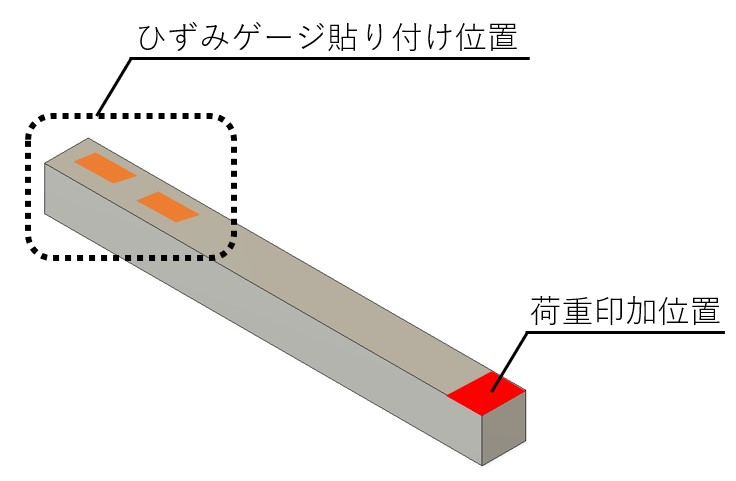
\includegraphics[width=6.0cm]{pic/hari.jpg}
    \caption{HDR1軸力覚センサのCADモデル}\label{fig:sensor}
  \end{center}
\end{figure}

\begin{table}[h]
  \caption{起歪体の寸法 [mm]}\label{tb:size}
  \begin{center}
   \begin{tabular}{ c c c c }
    \hline
     & Length & Width & Height  \\
    \hline
    Cantilever beam & 100 & 10 & 10  \\
    \hline   
   \end{tabular}
  \end{center}
 \end{table}

\subsection{ひずみゲージ貼り付け位置}
有限要素法シミュレーションによる起歪体のひずみ分布と, 
ひずみゲージの貼り付け位置をそれぞれFig.~\ref{fig:sim}, 
Fig.~\ref{fig:hizumi}に示す. 

ひずみゲージは被測定対象のひずみが伝達することにより抵抗変化が生じる
センシング素子である. 
ひずみの変化は大変微小であるため, ひずみゲージの貼り付け位置は
測定対象のよりひずみやすい部分に貼り付けることが求められる. 
よって有限要素法シミュレーションにより任意の荷重を印加, 
この時のひずみ分布をもとに貼り付け位置を決定した. 

また, このシミュレーション結果より得られた本センサの定格荷重と
定格荷重印加時の安全率のパラメータをTable~\ref{tb:kajuu}に示す.

\begin{table}[h]
  \caption{定格荷重と安全率}\label{tb:kajuu}
  \begin{center}
   \begin{tabular}{ c c }
    \hline
    定格荷重 $F$[N] & 安全率 \\
    \hline
    200.0 & 1.145 \\
    \hline   
   \end{tabular}
  \end{center}
 \end{table}

\begin{figure}[h]
  \begin{center}
    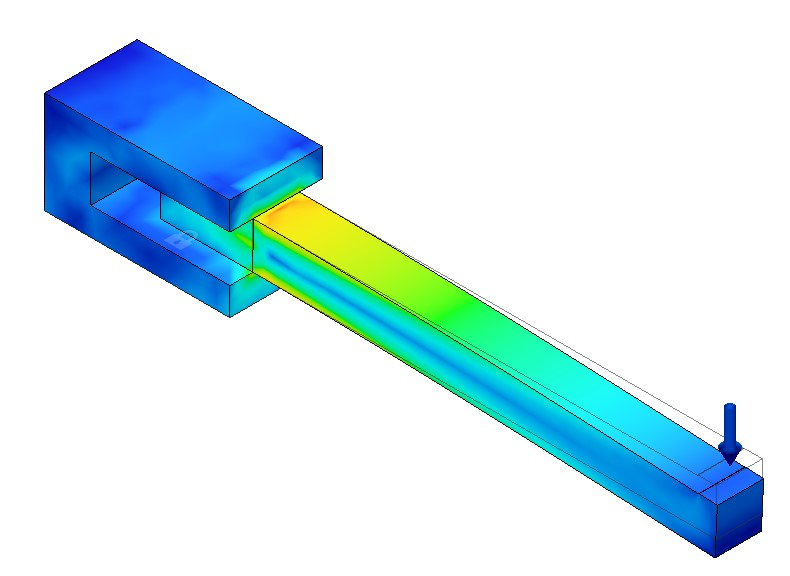
\includegraphics[width=6.0cm]{pic/simHizumi.jpg}
    \caption{有限要素法シミュレーションによる結果}\label{fig:sim}
  \end{center}
\end{figure}

\begin{figure}[h]
  \begin{center}
    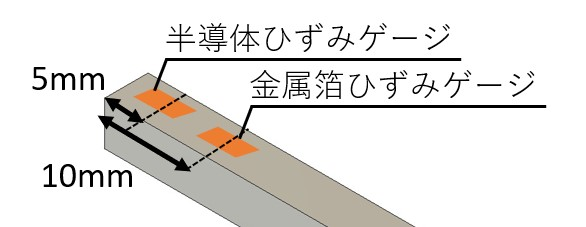
\includegraphics[width=6.5cm]{pic/hizumi.jpg}
    \caption{ひずみゲージの貼付位置}\label{fig:hizumi}
  \end{center}
\end{figure}